\subsection{Evaluation} 
\label{mazu-evaluation}

In this section, we use large-scale simulations with various topologies and
workloads to study 
our techniques' effectiveness in meeting the needs of management
applications that require low-latency control of data plane
state. We consider three applications: failover in a tunneled WAN, 
two-level responsive traffic engineering, and
MicroTE~\cite{benson2011microte}.
Our simulations leverage switch latency models derived from our measurements
(\secref{mazu-measure}).

\subsubsection{Failover in a Tunneled WAN}%Macro Benchmarks}%Flow Engineering} 
\label{mazu:fe_eval}

We first evaluate the effectiveness of flow engineering (\FE) and rule offload
(\RO) in the context of a control application that performs failover when a
link fails in  a tunneled WAN.


\tightparagraph{Topology} We use a simple full mesh (overlay) network of 25
nodes.  The tunnels between these nodes share the same physical network. Each
tunnel has between 5 and 10 intermediate switches. Per link capacity lies in
$[100,1000]$.

\tightparagraph{Workloads} We consider six workloads (\tabref{qosTable}). For
each workload,
we assign a popularity index (random number
within an internal) to each node. The number of flows between a pair
of nodes is proportional to the product of their popularities. Each flow
imposes a unit demand. At the start of our simulation, the traffic is routed
such that the maximum load on any link is minimized.

\tightparagraph{Table occupancy} We assume that the new rules being installed
upon failure (some of these could be updates to existing rules) all have the
same priority $P$. Further, we assume that the tunnel end-points already have
some lower priority rules, a subset of which are displaced by the new
rules. We randomly pick the number of such displaced rules within some
interval (defined for each workload in \tabref{qosTable}). For simplicity, we
assume that there are no dependencies across rules; we consider dependencies
in subsequent sections.

\newcommand{\sA}{{\em s1}}
\newcommand{\sB}{{\em s2}}
\newcommand{\sC}{{\em s3}}
\newcommand{\sD}{{\em s4}}
\newcommand{\sE}{{\em s5}}
\newcommand{\sF}{{\em s6}}

\begin{table}
\centering
\small
\tabcolsep=0.4em
\begin{tabular}{|c|c|c|c|c|}
\hline
\tabincell{c}{{\bf Work-}\\{\bf load}} & 
\tabincell{c}{{\bf Popularity}\\{\bf index}} &
\tabincell{c}{{\bf Popularity} \\{\bf index for high}\\{\bf prio. traffic}} & 
\tabincell{c}{{\bf \# of flows}\\{\bf between any}\\{\bf pair of nodes}} & 
\tabincell{c}{{\bf \# of low}\\{\bf prio. rules}\\{\bf in flowtable}}\\ 
\hline
\sA 
    & \multirow{3}{*}{\tabincell{c}{1-10}} 
    & \multirow{3}{*}{\tabincell{c}{1-5}} 
    & \multirow{3}{*}{\tabincell{c}{Avg: 50\\Max: 100}} 
    & 0-50 \\ \cline{1-1} \cline{5-5}
\sB & & & & 100-200 \\ \cline{1-1} \cline{5-5}
\sC & & & & 300-500 \\ \hline
\sD 
    & \multirow{3}{*}{\tabincell{c}{1-20}} 
    & \multirow{3}{*}{\tabincell{c}{1-7}} 
    & \multirow{3}{*}{\tabincell{c}{Avg: 200\\Max: 400}} 
    & 0-50 \\ \cline{1-1} \cline{5-5}
\sE & & & & 100-200 \\ \cline{1-1} \cline{5-5}
\sF & & & & 300-500 \\ \hline
\end{tabular}
\caption{Workloads used in simulation}{\label{qosTable}}
\end{table}


To simulate failures we randomly select a tunnel in the mesh and fail it.  On
a link failure, about 70 flows are rerouted for low traffic workloads
(\sA-\sC) and 220 for high traffic workloads (\sD-\sF).  We assume that there
is enough spare capacity in the network to reroute the affected flows. All
rerouted flows are treated as new flows.  

We consider three techniques for rerouting: (1) {\em Base case}, which
reroutes the affected flows while minimizing the maximum link load, ignoring
setup latencies.
(2) Flow engineering ({\em \FE}), which selects paths for affected flows such
that flow installation latency is minimized (\secref{mazu-floweng}). (3) Flow
engineering plus rule offloading ({\em \FE+\RO}), which applies \FE and
then offloads a set of rules from the tunnel end-nodes to at most $k=3$ next
hop switches per tunnel (\secref{mazu-offload}). 

In all cases, we assume that one-shot consistent updates~\cite{reitblatt2012abstractions} are employed to install routes. Thus, our metric of interest is the {\em worst case latency incurred at any switch to install all new/modified routes at the switch.}

We simulate with both \BroadcomOne and Intel, assuming all switches in the
network are from the same vendor. \figref{failoverResults} shows the
latencies with \BroadcomOne switches for the three techniques. For the lowest
volume workload, the base case incurs a latency of 720ms, whereas \FE improves
this to 259ms and \FE+\RO to 133ms. These improvements are crucial, especially
for latency sensitive interactive applications.

For the remaining workloads, base case latency varies between 2 and 14s.
Using \FE offers 22-35\% improvement, but using \FE together with \RO leads to
nearly a {\em factor of 3} improvement in all cases. Note that the gains can
be improved further by: (1) leveraging more core switches for offload, and (2)
providing a modest amount of reserved capacity for highly critical traffic,
so that during failures the number of flows whose routes have to be
recomputed is small and the rerouted non-critical flows can tolerate modest
amounts of downtime or congestion. In other words, 
\FE and \RO provide operators
additional flexibility in designing schemes to better meet failover
requirements in their networks. 

\figref{runtime} shows the runtime overhead of FE and RO. FE takes $<13ms$ for
all workloads, while FE+RO takes up to 1.4s. However, even after taking into
account this overhead, the net latency benefit of FE+RO for BCM-1.0 switches is still
$\approx$0.3s to 6.6s, depending on workload. Furthermore, we focused on
correctness, not efficiency, in designing our simulator, so there is still
ample opportunity for improvement.
    
We also run our simulation with the \Intel model. Since all rules we insert
have the same priority, and the \Intel switch does not impose rule
displacement in such situations, the latency is purely driven by the maximum
number of rules inserted at any switch. In our simulations, this is almost
always at source end-point on a failed tunnel. Since both base case and \FE
are equally impacted by this, we don't see any improvement from using \FE.
However, \RO still applies, as rules can be offloaded to core switches---we
see an improvement of {\em over 2X} (324ms to 129ms).


\begin{figure}[!tb]
\centering
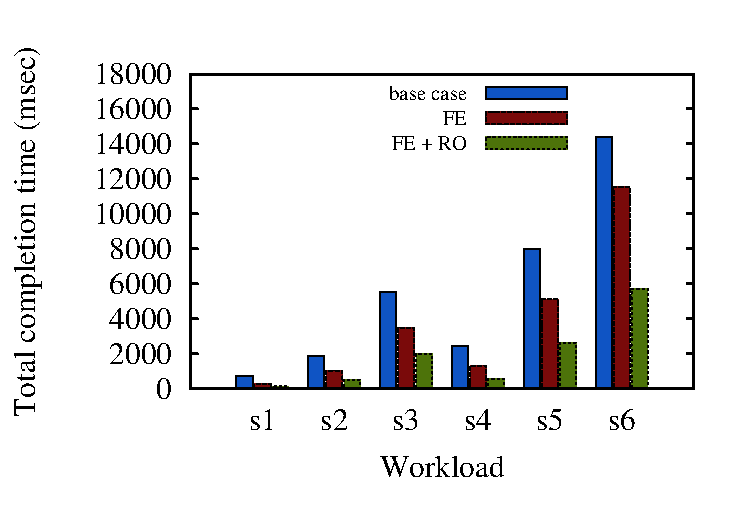
\includegraphics[width=0.55\textwidth]{figures/mazu/Failover-eps-converted-to.pdf}
\caption{Worst case flow setup time of affected flows in the failover
scenario with \BroadcomOne switches}\label{failoverResults}
\end{figure}

\begin{figure}
\centering
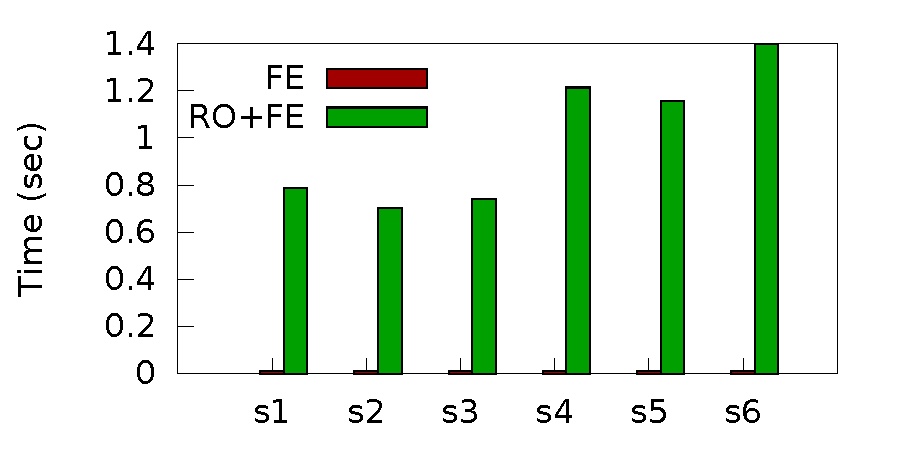
\includegraphics[width=0.55\textwidth]{figures/mazu/fe_ro_runtime.pdf}
\caption{Running time for FE and RO}
\label{runtime}
\end{figure}

\subsubsection{Two-level Responsive Traffic Engineering} 
Next, we evaluate the effectiveness of \FE and \RO in the
context of a control application that performs two-level responsive traffic
engineering. This application simultaneously routes two classes of
traffic---high and low priority---over the same network according to
different objectives. For low priority traffic, the objective is to minimize
the overall link utilization of the network due to this traffic; we install
coarse grained (wildcard) rules to route this traffic.  The objective for
high priority traffic is to minimize the overall link latency; we install
fine grained high priority rules to route this traffic. We first route the
low priority traffic, and then route the high priority traffic using the
remaining network capacity. We assume both categories of traffic can be
accommodated without causing any congestion. 

We use the same topology and workloads described in \secref{mazu:fe_eval}.
However, for high volume workloads (\sD-\sF) the volume of high priority and
low priority traffic between any two overlay nodes is about 17 and 200 flows,
respectively, and for low volume workloads (\sA-\sC) the volume is about 12
and 50 flows, respectively.

A network's ability to meet SLAs for each traffic class depends on how
quickly the network can establish routes when requests for both classes
arrive close in time.
\figsref{qos_Results}{qos_intelResults} show the total completion time using
\BroadcomOne and \Intel switches, respectively, with and without our
techniques. The base case has a significantly high flow set up time when the
number of low priority rules in the table are high: as high as 80s for
\BroadcomOne. This implies that ignoring flow setup latency can cost traffic
engineering dearly in terms of being responsive.  For low volume workloads
(\sA-\sC) the factor of improvement from just \FE is about 2.5X for
\BroadcomOne and 1.8X for \Intel, and with \FE+\RO it's about 5X for
\BroadcomOne and 4X for \Intel. We observe similar speedups for high volume
workloads (\sD-\sF). 

\begin{figure*}[!t]
\centering
        \begin{subfigure}[b]{0.40\textwidth}
                \centering
		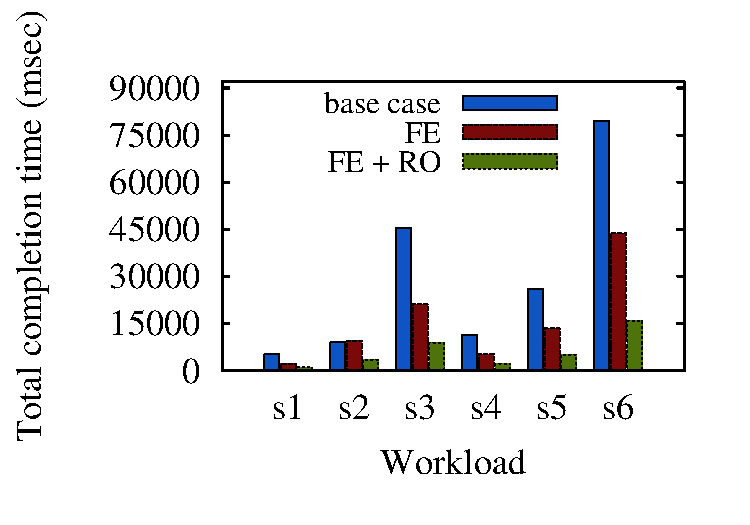
\includegraphics[width=\textwidth]{./figures/mazu/qos-eps-converted-to.pdf}
		\caption{Latency on \BroadcomOne switch}
		\label{qos_Results}
	\end{subfigure}
        \begin{subfigure}[b]{0.40\textwidth}
                \centering
		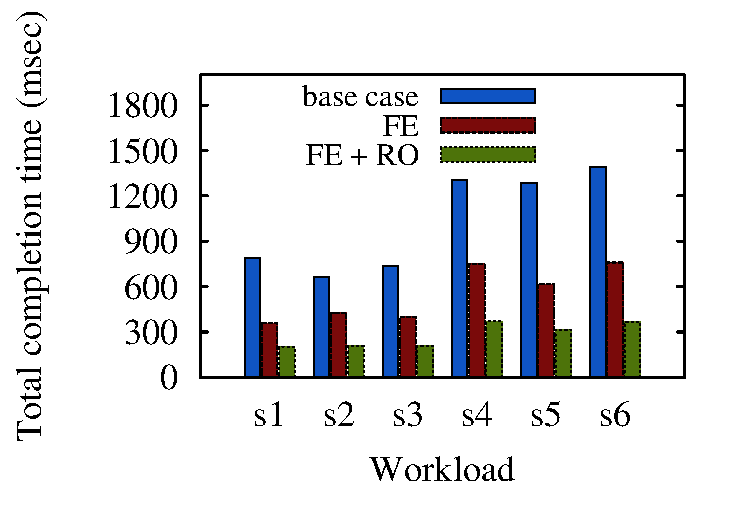
\includegraphics[width=\textwidth]{./figures/mazu/qos_intel-eps-converted-to.pdf}
		\caption{Latency on \Intel switch}
		\label{qos_intelResults}
	\end{subfigure}
	\caption{Worst case flow set up time in the two level traffic
    engineering scenario} 
	\label{qosResults}
\end{figure*}

\subsubsection{MicroTE}
MicroTE~\cite{benson2011microte} leverages the partial and short term
predictability of a data center traffic matrix to perform traffic engineering
at small time-scales. As noted in \secref{mazu-floweng}, \FE does not apply to
MicroTE since routes span a single tunnel and route changes all happen at a
single switch. Thus, MicroTE can only benefit from \RO, the extent of which we
now study.

We consider the following simple data center topology: we use a three-level FatTree topology~\cite{fattree} with degree 8, containing 128 servers connected by 32 edge, 32 aggregate, and 16 core switches.
We assume that the traffic rate between a pair of servers is derived from a
Zipfian distribution. \figref{microteResults} shows the rule installation
completion time. We see that \RO provides a 2X improvement (400ms to 200ms)
assuming the \BroadcomOne switch. Given the time-scales of predictability
considered, this can help MicroTE leverage traffic predictability longer,
thereby achieving more optimal routing. The improvement with \Intel is 1.6X
(80ms to 48ms).


\begin{figure}[!tb]
\centering
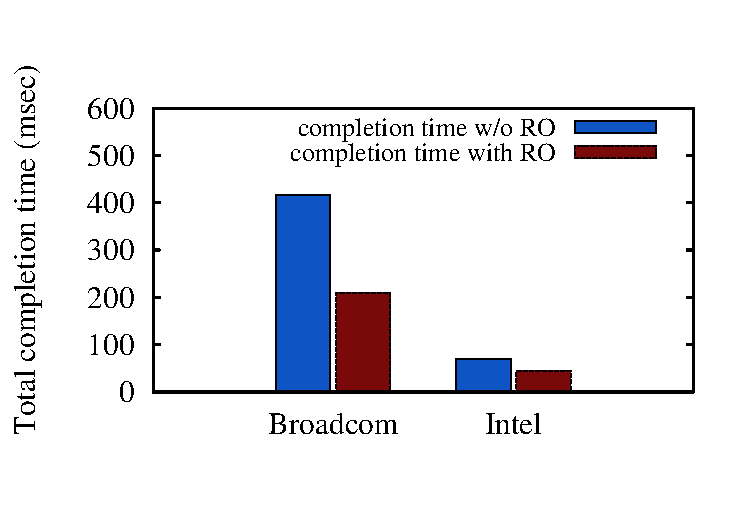
\includegraphics[width=0.55\textwidth]{./figures/mazu/MicroTE_Compl-eps-converted-to.pdf}
\caption{Flow setup time of MicroTE with and without \RO in a Fat Tree (k=8) topology}
\label{microteResults}
\end{figure}

